\documentclass[12pt, oneside]{article}
\usepackage[letterpaper, margin=1in, headsep=0.5in]{geometry}
\usepackage[english]{babel}
\usepackage[utf8]{inputenc}
\usepackage{amsmath}
\usepackage{amsfonts}
\usepackage{amssymb}
\usepackage{tikz}
\usetikzlibrary{quotes, angles}
\usepackage{graphicx}
%\usepackage{pgfplots}
%\pgfplotsset{width=10cm,compat=1.9}
%\usepgfplotslibrary{statistics}
%\usepackage{pgfplotstable}
%\usepackage{tkz-fct}
%\usepackage{venndiagram}
\usepackage{multicol}


\usepackage{fancyhdr}
\pagestyle{fancy}
\fancyhf{}
\rhead{\thepage \\Name: \hspace{1.5in}.\\}
\lhead{BECA / Dr. Huson / Geometry 10th Grade\\* Unit 4: Parallels and transversals \\ 30 October 2019}

\renewcommand{\headrulewidth}{0pt}

\begin{document}
\subsubsection*{4.9 Homework: Isosceles triangles}
  \begin{enumerate}

\item Given isosceles $\triangle ABC$ with $\overline{AC} \cong \overline{BC}$. On the diagram mark the congruent line segments with tick marks.
\begin{center}
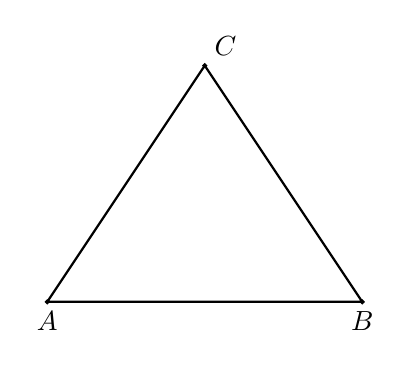
\begin{tikzpicture}[scale=0.5]
  \draw [thick](0,0)--(8,0)--(4,6)--(0,0);
  \draw [fill] (0,0) circle [radius=0.05] node[below]{$A$};
  \draw [fill] (8,0) circle [radius=0.05] node[below]{$B$};
  \draw [fill] (4,6) circle [radius=0.05] node[above right]{$C$};
\end{tikzpicture}
\end{center}

\item Given $\triangle ABC$ with $\overline{AC} \cong \overline{BC}$. $AC=5x+7$ and $BC=3x+17$. Find $AC$.
\begin{flushright}
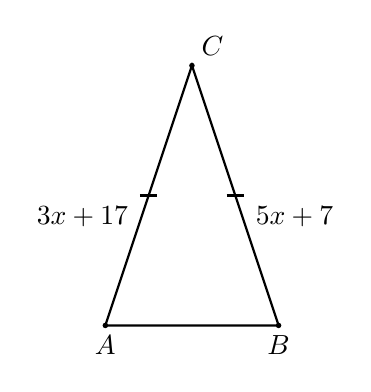
\begin{tikzpicture}[scale=0.55]
  \draw [thick](0,0)--(4,0)--(2,6)--(0,0);
  \draw [fill] (0,0) circle [radius=0.05] node[below]{$A$};
  \draw [fill] (4,0) circle [radius=0.05] node[below]{$B$};
  \draw [fill] (2,6) circle [radius=0.05] node[above right]{$C$};
  \draw [thick] (0.8,3)--(1.2,3); %tick mark
  \draw [thick] (2.8,3)--(3.2,3); %tick mark
  \node [right] at (3.25,2.5){$5x+7$};
  \node [left] at (0.75,2.5){$3x+17$};
\end{tikzpicture}
\end{flushright} \vspace{1cm}

\item Given isosceles $\triangle ABC$ with $\overline{AC} \cong \overline{BC}$, $m\angle A = 12x$, and $m\angle B = 42$. Find $x$. Find $m\angle C$.
\begin{flushright}
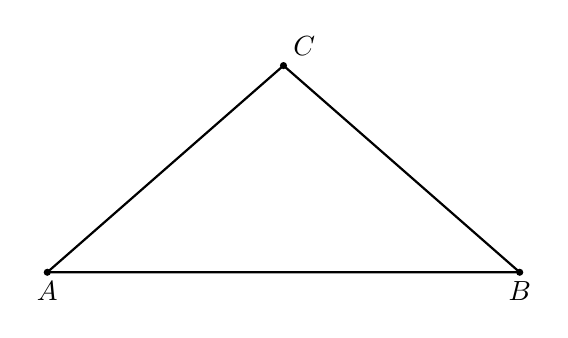
\begin{tikzpicture}[scale=0.75]
  \draw [thick](0,0)--(8,0)--(4,3.5)--(0,0);
  \draw [fill] (0,0) circle [radius=0.05] node[below]{$A$};
  \draw [fill] (8,0) circle [radius=0.05] node[below]{$B$};
  \draw [fill] (4,3.5) circle [radius=0.05] node[above right]{$C$};
\end{tikzpicture}
\end{flushright}

\newpage

\item Given isosceles $\triangle RSU$ with $\overline{UR} \cong \overline{US}$. If $m\angle UST=130$ find $m\angle U$.
\begin{flushright}
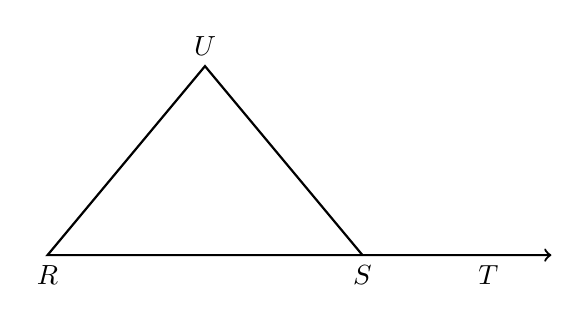
\begin{tikzpicture}[scale=0.8]
  %\draw [->, thick] (0,0)--(5,5);
  \draw [<-, thick] (8,0)--
    (7,0) node[below]{$T$}--
    (0,0) node[below]{$R$}--
    (2.5,3) node[above]{$U$}--
    (5,0) node[below]{$S$};
\end{tikzpicture}
\end{flushright} \vspace{2cm}


\item Given parallel lines $\overleftrightarrow{AB} \parallel \overleftrightarrow{CDE}$ with $\overline{AC} \cong \overline{AD}$. If $m\angle BAD=70$ find $m\angle ACD$.
\begin{flushright}
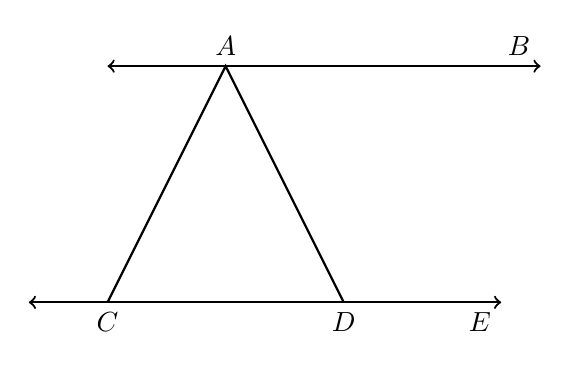
\begin{tikzpicture}
  \draw [<->, thick] (1,3)--(6.5,3) node[above left]{$B$};
  \draw [<->, thick] (0,0)--
    (5,0)--
    (6,0) node[below left]{$E$};
  \draw [-, thick] (1,0) node[below]{$C$}--
    (2.5,3) node[above]{$A$}--
    (4,0) node[below]{$D$};
\end{tikzpicture}
\end{flushright} \vspace{1.5cm}


\item Given $\overrightarrow{BA} \perp \overrightarrow{BC}$, $m \angle ABD = 4x$, and $m \angle DBC = 2x-12$. Find $m \angle DBC$. \\[0.5cm]
For full credit, show the check using both angle measures.
  \begin{flushleft}
  \begin{tikzpicture}[scale=1.3]
    \draw [<->, thick] (0,3)--(0,0)--(5,0);
    \draw [->, thick] (0,0)--(3.5, 2);
    \draw [-, thin] (0, 0.4)--(0.4, 0.4)--(0.4, 0);
    %\node at (3,.4){1};
    %\node at (6,-.6){2};
    \draw [fill] (0,0) circle [radius=0.05] node[below]{$B$};
    \draw [fill] (0,2) circle [radius=0.05] node[left]{$A$};
    \draw [fill] (4,0) circle [radius=0.05] node[below]{$C$};
    \draw [fill] (2.625, 1.5) circle [radius=0.05] node[below]{$D$};
  \end{tikzpicture}
  \end{flushleft}
  \vspace{3cm}


  \end{enumerate}

\end{document}
